\section{Graficzny interfejs użytkownika}
Graficzny interfejs użytkownika stanowi desktopowa aplikacja okienkowa, której głównym elementem jest panel zakładek. Każda z zakładek reprezentuje wizualizację osobnego algorytmu planowania ruchu robotów.

Z myślą o spopularyzowaniu i rozpowszechnieniu opracowanych algorytmów, elementy interfejsu użytkownika (takie, jak etykiety lub przyciski) posiadają tekst w języku angielskim.

Pod każdą z zakładek aplikacji układ wizualny jest podobny. Poniżej opisano graficzny interfejs użytkownika wspólny dla wszystkich zakładek (por. rys. \ref{fig:robopath-ui-whca}).

Po prawej stronie znajduje się panel przycisków akcji oraz panel rozwijanych właściwości z konfiguracją parametrów mapy oraz symulacji. Natomiast po lewej stronie wyświetlany jest obecny stan mapy i położenie robotów mobilnych. Mapa wyświetlana jest z zaznaczeniem linii siatki pól obrazujących liczbę pól na mapie. Przeszkody wyświetlane są jako czarne kwadraty, zaś roboty jako kolorowe wypełnione koła.
Kliknięcie prawym przyciskiem myszy (również z możliwością ciągłego przytrzymania) powoduje wstawienie lub usunięcie przeszkody na mapie w odpowiednich polach.
Punkty docelowe, do których podążąją roboty wyświetlane są jako krzyżyki w kolorze takim samym, jaki został przypisany do robota. Liczba robotów nie jest ograniczona przez aplikację. Aby odróżniać roboty między sobą, każdy robot otrzymuje inny kolor wynikający z równomiernego podziału na liczbę robotów zakresu barwy (ang. {\it hue}) z palety HSV.

Okno aplikacji jest skalowalne i w pełni responsywne. Po zmianie rozmiaru okna przez użytkownika rozmiar mapy dopasowuje się do maksymalnego obszaru, jaki może zająć (z zachowaniem proporcji wymiarów mapy).

Symulacja ruchu robotów rozpoczyna się, gdy tylko zostanie wyznaczony punkt docelowy dla robota. Dzięki temu, że wykonywanie obliczeń planowania tras zostało przeniesione do osobnych wątków, uzyskano płynność animacji ruchu robotów mobilnych. Uniknięto również problemu braku odpowiedzi okna interfejsu użytkownika podczas planowania trajektorii.

\subsection{Metoda pól potencjałowych}
Na pierwszej zakładce "Potential fields" w oknie aplikacji przedstawiona jest wizualizacja metody pól potencjałowych.

\begin{figure}
	\centering
	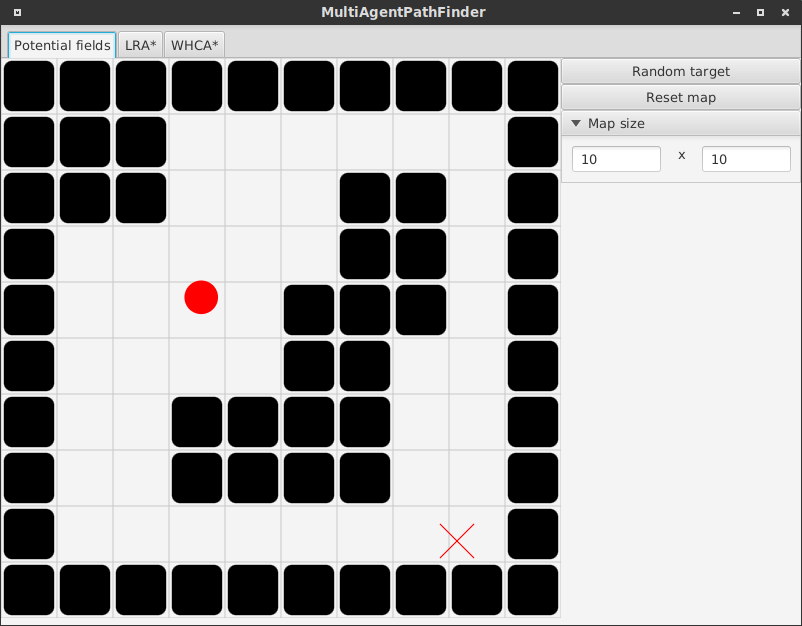
\includegraphics[width=0.8\columnwidth]{img/robopath/ui-fields}
	\caption{Zrzut ekranu aplikacji w trakcie wizualizacji metody pól potencjałowych.}
	\label{fig:robopath-ui-fields}
\end{figure}

Na panelu konfiguracji parametrów, użytkownik może wybrać dowolny rozmiar mapy, podając szerokość i wysokość wyrażone w liczbie pól.
Po naciśnięciu przycisku "Reset map" tworzona jest nowa mapa o zadanych rozmiarach, natomiast pozycja początkowa robota zostaje wylosowana.
Naciśnięcie przycisku "Random target" powoduje wyznaczenie losowego punktu na mapie jako celu dla robota i rozpoczęcie podążąnia za nim.

Klikając lewym przyciskiem myszy na mapie, użytkownik może manualnie wskazać punkt docelowy dla robota.
Planowanie i symulacja ruchu robota odbywa się w trybie ciągłym. Robot nie jest ograniczony zdyskretyzowaną siatką pól na mapie, jego przestrzeń poruszania się jest ciągła.

\subsection{Local-Repair A*}
\label{ch:app-lra}
Pod kolejną zakładką "LRA*" w oknie aplikacji dostępna jest wizualizacja metody algorytmu bazującego na A* z lokalną detekcją i rozwiązywaniem kolizji.

Na panelu konfiguracji parametrów w sekcji "Map size", użytkownik może wybrać dowolny rozmiar mapy, podając szerokość i wysokość wyrażone w liczbie pól.
Po naciśnięciu przycisku "Reset map" tworzona jest nowa, pusta mapa o zadanych rozmiarach.
W sekcji "Robots" użytkownik wybiera liczbę robotów (do automatycznego rozmieszczenia) oraz ma możliwosć zaznaczenia opcji "auto-assign next target", co skutkuje automatycznym wyznaczaniem kolejnego punktu docelowego, dla robota, który dotarł do poprzedniego celu.
Przycisk "Generate maze" pozwala na wygenerowanie labiryntu przy użyciu generatora map (por. \ref{ch:mazegen}).
Przycisk "Place robots" usuwa wszystkie roboty z mapy i umieszcza na niej wybraną przez użytkownika liczbę robotów w losowych miejscach na mapie (z pominięciem pól zajętych przez przeszkody oraz inne roboty).
Przycisk "Random target" losuje punkty docelowe dla wszystkich robotów. Każdy z agentów otrzymuje inny punkt docelowy (nie będący przeszkodą), do którego zmierza. Nadanie punktów docelowych powoduje rozpoczęcie planowania trajektorii i symulację ruchu agentów.

Klikając lewym przyciskiem myszy na mapie, użytkownik może utworzyć nowego robota. Nowemu agentowi zostaje przydzielony punkt docelowy w miejscu, w którym lewy przycisk myszy został zwolniony.
Dodatkowo pokazywane są zaplanowane ścieżki dla każdego robota. Wyświetlane są jako linie łamane w kolorze takim samym, jaki odpowiada robotowi.
Nad robotem, w jego aktualnym położeniu wyświetlany jest jego numer (identyfikator).

\begin{figure}
	\centering
	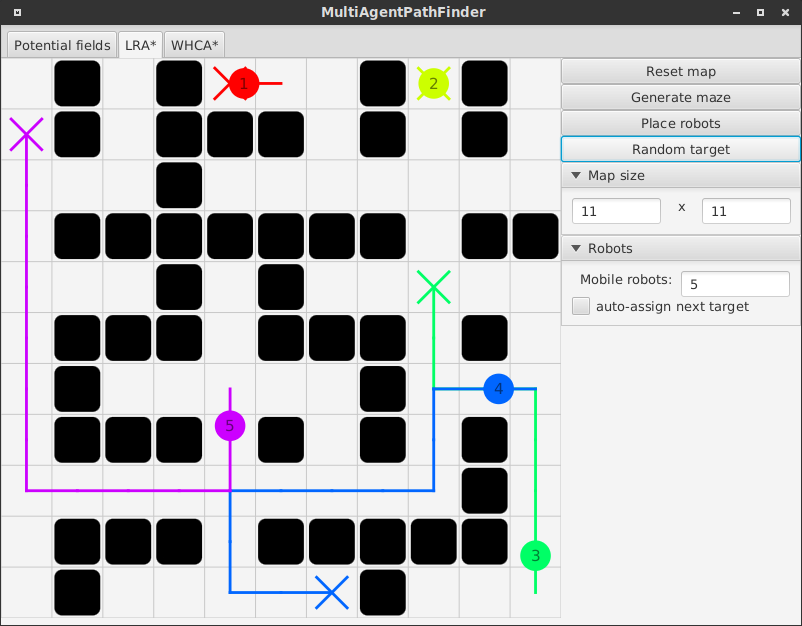
\includegraphics[width=0.8\columnwidth]{img/robopath/ui-lra}
	\caption{Zrzut ekranu aplikacji w trakcie wizualizacji metody Local-Repair A*.}
	\label{fig:robopath-ui-lra}
\end{figure}


\subsection{Windowed Hierarchical Cooperative A*}
Pod ostatnią zakładką "WHCA*" w oknie aplikacji dostępna jest wizualizacja metody kooperacyjnego planowania tras dla wielu robotów z wykorzystaniem wariantu metody WHCA*3 z dynamicznym przydziałem priorytetów oraz skalowaniem okna czasowego (por. \ref{ch:alg-priorities-allocation}).

Interfejs użytkownika jest praktycznie taki sam, jak w przypadku opisanej metody LRA* (por. \ref{ch:app-lra}).
Różni się obecnością dodatkowej sekcji "WHCA*" na panelu konfiguracji z polem "Time window", które pozwala na zmianę początkowej wielkości okna czasowego dla algorytmu WHCA*. W wyniku dynamicznego przydzielania priorytetów wielkość ta może zostać zwiększana automatycznie podczas symulacji.
Dodatkowy przycisk "Restore positions" pozwala na cofnięcie stanu robotów do momentu, tuż przed rozpoczęciem symulacji (zaraz po przydzieleniu punktów docelowych). Pozwala to na ponowną obserwację przebiegu symulacji dzięki przywróceniu położenia i stanu agentów.

Nad robotem, w jego aktualnym położeniu wyświetlany jest jego numer (identyfikator) oraz priorytet (oddzielony kropką). Priorytet może być zmienny w trakcie symulacji (w przeciwieństwie do identyfikatora). Początkowo robot zawsze ma priorytet równy identyfikatorowi. Większa wartość priorytetu względem pozostałych oznacza pierwszeństwo uwzględniane podczas planowania tras.

\begin{figure}
	\centering
	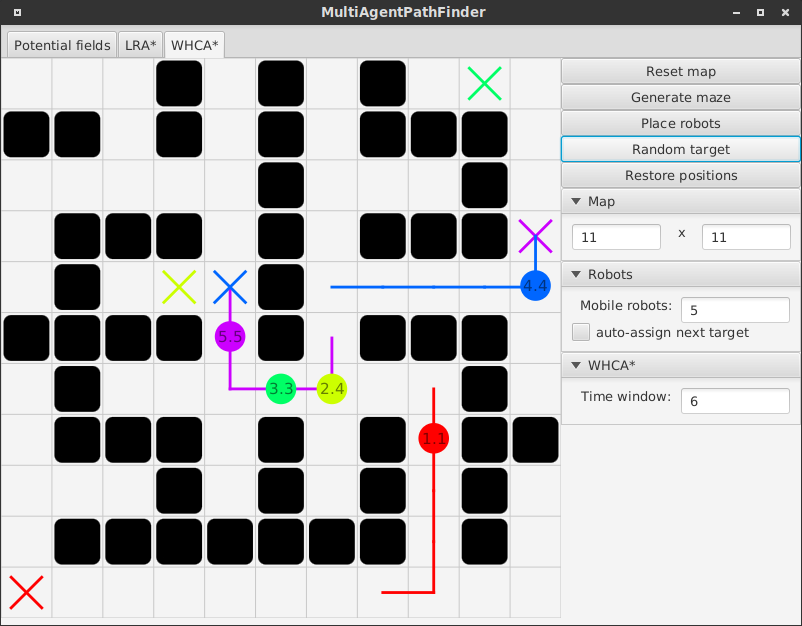
\includegraphics[width=0.8\columnwidth]{img/robopath/ui-whca}
	\caption{Zrzut ekranu aplikacji w trakcie wizualizacji metody Windowed Hierarchical Cooperative A*.}
	\label{fig:robopath-ui-whca}
\end{figure}
